\section{Explication du fonctionnement des différents composants}
    \subsection{Liste des différents composants utilisés}
    La carte Raspberry est reliée à différents composants ci dessous :    
	    \begin{itemize}
            \item $\bullet$ \textbf{1 capteur à ultrason} (situé sur le devant du robot) permet de détecter les potentiels obstacles se plaçant devant le robot.
            \item $\bullet$ \textbf{4 capteurs suiveurs de ligne} permettent au robot de suivre la ligne noir en la détectant continuellement. Concernant le placement des capteurs, il y en a 3 à l'avant (1 au centre, 1 à gauche, 1 à droite) et 1 à l'arrière (centré avec le capteur placé à l'avant au centre).
            \item $\bullet$ \textbf{2 moteurs} (situés à l'arrière) permettent au robot de se déplacer.
            \item $\bullet$ \textbf{1 carte moteur  } permet le contrôle des moteurs.  
            \item $\bullet$ \textbf{1 écran LCD} (situé sur le dessus du robot) permet l'affichage des commandes du robot en cours d'exécution.
            \item $\bullet$ \textbf{1 buzzer} (situé à l'arrière du robot) permet d'émettre un son lors de l'arrêt d'urgence.
            \item $\bullet$ \textbf{1 batterie } permet d'alimenter en électricité la carte Raspberry.
            \item $\bullet$ \textbf{2 piles } permettent d'alimenter les moteurs en électricité.
            \item $\bullet$ \textbf{1 bouton } (situé à l'arrière du robot) permet d'ouvrir ou fermer le circuit électrique et ainsi démarrer les moteurs.
            \item $\bullet$ \textbf{1 LED } (situé à l'arrière du robot) permet d'indiquer l'état de charge de la batterie.
        \end{itemize} 
    \vspace{5mm}
     
    \subsection{Capteur à ultrason} 

        Le capteur à ultrason envoie un signal sonore à l'aide d'un émetteur, puis le signal émis va percuter un obstacle et ainsi être réfléchi. Un capteur a ultrason faisant partie du dispositif va permettre de récupérer le signal réfléchi. Ainsi pour évaluer la distance entre l'objet et le capteur il suffit d'appliquer la formule suivante : \\ \\$\frac{360 \times temps \times V_{son}}{2} = distance$ \\ \\Le temps (en seconde) et la distance (en mètre) et $V_{son}$ la vitesse du son dans l'air (344m/s), permettent de déterminer à quelle distance se situe l'objet. Il ne reste ensuite plus qu'à programmer à partir de quelle distance minimale le robot doit s'arrêter. La distance minimale retenue est de 15cm.


    \subsection{Capteurs de ligne} 

        Les capteurs de ligne permettent de détecter une ligne sombre sur un fond clair et inversement. Les capteurs sont calibrés grâce à un potentiomètre situé sur le capteur. Ces capteurs possèdent 2 modes de sorties:
        
        \begin{itemize}
            \item Un mode de sortie analogique: plus la ligne est foncée, plus la valeur renvoyée est grande.
            \item Un mode de sortie tout ou rien: si la couleur du fond est supérieure au seuil défini par le potentiomètre alors le capteur renvoie 1, sinon il renvoie 0.
        \end{itemize} 
        \vspace{5mm}
        \ \ \ Dans notre cas, nous avons utilisé le mode tout ou rien pour détecter une ligne. 

    \subsection{Bouton on/off}
    
        Le bouton on/off (activation manuelle) est branché en série sur le circuit, il sert d'interrupteur afin de ne pas alimenter les moteurs lorsque le robot n'est pas en fonctionnement. Cela permet d'économiser de la batterie. 

    \subsection{LED}

        La LED s'allume quand la valeur du courant qui circule à l'interieur est supérieure à un certain seuil défini en fonction de la couleur de la LED. Dans notre cas la LED est rouge donc elle nécessite une tension comprise entre 1.8V et 2.1V pour s'allumer. Au dessus de cette limite, la led cesse de fonctionner et devient inutilisable. En dessous de cette limite, la LED ne s'allume pas (ou très peu) car elle agit comme une diode. 

    \subsection{Carte moteur}

        La carte moteur permet de contrôler les moteurs. Elle prend en entrée une alimentation externe et une tension définit par la formule suivante: \\ \\ $\frac{1024 \times vitesseMoteur}{100}$ \\ \\ La vitesse du moteur est en pourcentage (de 0 à 100) de la vitesse maximale du moteur. La carte moteur renvoie en sortie une tension et un courant adapté pour le moteur selon ses entrées. Ainsi grâce à cette formule, nous sommes capables de définir la vitesse de rotation du moteur, mais aussi d'activer ou de désactiver un moteur afin de réaliser un virage par exemple.
        
    \subsection{Buzzer}

        Le buzzer émet un signal sonore lorsqu'il reçoit une tension en entrée de 3.3V. 

    \subsection{Ecran LCD}

        L'écran LCD possède différents pixels qu'il faut mettre à jour afin d'afficher le contenu voulu. Pour le mettre à jour, on utilise les ports SDA et SCL de l'écran pour communiquer avec la carte Raspberry. Dans notre cas, l'écran LCD affichera les ordres en cours et la détection d'intersection. 
    
    \subsection{La carte Raspberry}

        C'est la carte électronique principale du robot ayant un OS intégré (linux). Elle est capable d'éxécuter des lignes de codes grâce à une barette de RAM et un processeur intégré. Elle possède en entrée des GPIOs qui permettent de contrôler des éléments externes comme le buzzer ou la carte moteur. Elle est alimentée via un câble USB-C et possède des ports pour brancher un écran, un clavier, une souris ... Une carte réseau est également intégrée, ce qui permet de contrôler la carte à distance via le protocole SSH. Le stockage est assérée via une carte micro-SD. 
        
        \textbf{Ci-dessous une vision simple du robot, pour comprendre sa structure globale}
        \begin{figure}[!h]
            \center 
            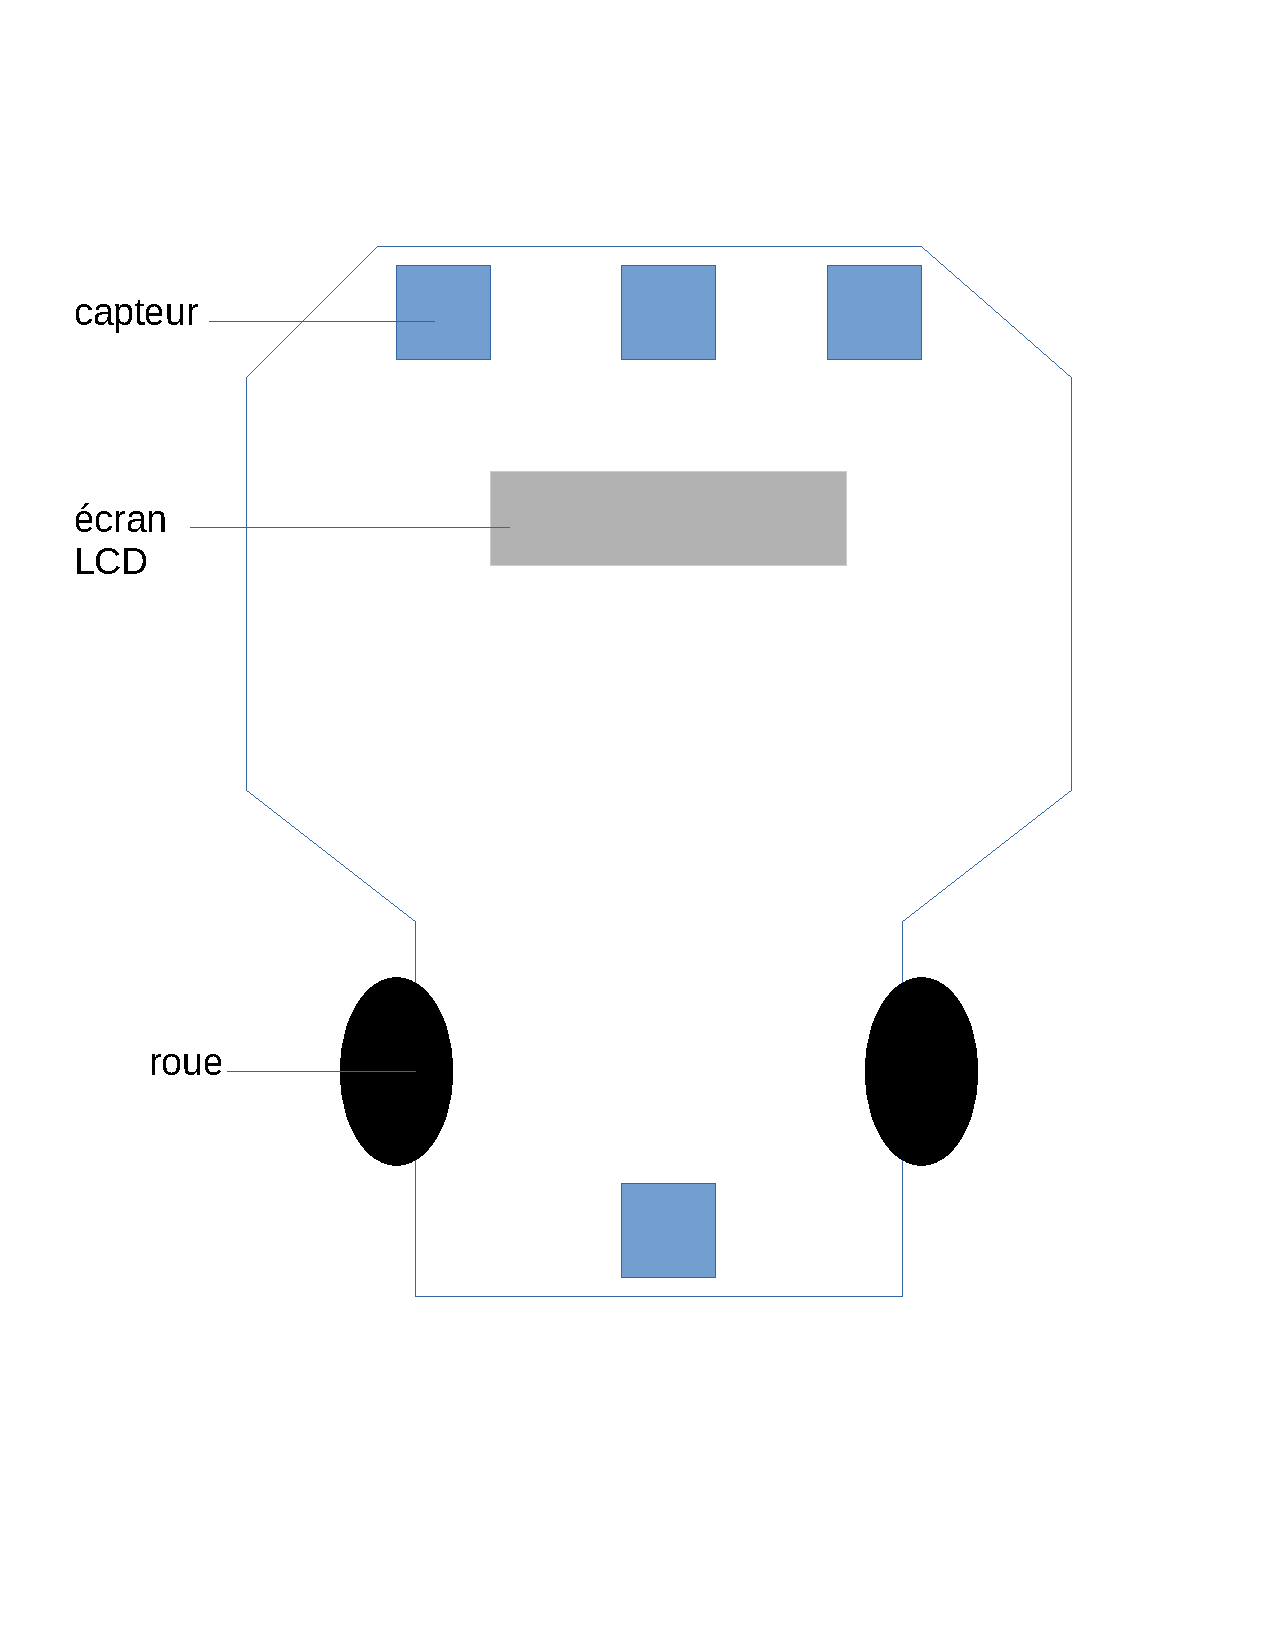
\includegraphics[width=0.9\linewidth]{imagesRapport/schema_simplifie_robot.pdf} 
            \caption{Schéma simplifié du robot}  
            \label{fig:analyse}
        \end{figure}
    
    
